\documentclass{CST_CryptoIntro}
\usepackage{indentfirst}
% ===== 封面配置 =====
\reportCourse{密码分析学实验报告}
\reportLogo{figures/logo_sduWithText.jpg}
\reportName{邱泽辉、江李阳、王健一}
\reportID{202400460046、202400460042、202400460037}
\reportMajor{密码科学与技术}

% ===== 页眉配置 =====
\headerLeft{密码分析学}
\headerRight{第二次实验实验报告}

\begin{document}

% ===== 封面 =====
\maketitle
\thispagestyle{fancy}
\newpage

% ===== 目录 =====
\tableofcontents
\newpage

% ===== 正文 =====
% \section{实验目的}
\section{组员分工}
\begin{itemize}
    \item 江李阳：完成任务一、二、三的代码和对应实验报告章节内容的撰写。
    \item 王健一：完成任务四、五的代码和实验报告对应章节内容的撰写。
    \item 邱泽辉：完成任务一、二、三的代码撰写，实验报告最终检查润色。
\end{itemize}

% 实验环境
\section{实验环境}
\begin{itemize}
    \item 硬件环境：13th Gen Intel(R) Core(TM) i5-13420H 处理器，12 个逻辑处理器，主频约为 2.1 GHz；内存 16 GB。
    \item 软件环境：Windows 操作系统、MacOS,Visual Studio Code 集成开发环境。
    \item 编程语言：Python 3.14。
\end{itemize}

% 实验原理
\section{实验原理}

\subsection{差分路线}
$i$轮差分路线是指对输入对$(X,X')$，在$i$轮加密过程中满足对应第$j$轮的一对输出值$(Y,Y')(1
le j \le i)$，满足$\Delta X = X \oplus X' = \beta_0$，$\Delta Y =  \oplus Y' = beta_j(1 \le j \le i)$，则称
$$
 \beta_0  \to \beta_1 \to \dots \to \beta_i 
$$
为一条$i$轮差分路线。假设密码算法的输入$X$和各轮密钥$K_i$的取值是相互独立且均匀分布的，对于满足输入差分为$beta_0$、输出差分为$\beta_i$(显然满足输入差分为$\beta_0$的明文不只一对)的$i$轮差分路线概率为$DP(\beta_0 \to \beta_i)$,其概率为各轮差分路线概率的乘积
$$
\text{DP}(\beta_0 \to \beta_1 \to \dots \to \beta_i)  = \prod_{(j=1)}^{i}\text{DP}(\beta_{j-1} \to \beta_j)
$$
注意这里差分路线是精确记录了包括起始、最终结果和中间每一种状态的一条路线。影响上述$i$轮差分路线的概率的主要因素是输入差分非零的$S$盒的个数以及输入差分非零的$S$盒对应的输出差分(因为当前轮$S$盒的输出即为下一轮$S$盒的输入)，其中输入非零的$S$盒被称为活跃$S$盒。

\subsection{差分}
$i$轮差分是指给定了输入差分$\beta_0$和$i$轮加密后的输出差分$\beta_i$，满足上述条件的称为$i$轮差分。与$i$轮差分路线相比，它不指定加密的中间状态。因此，对于$i$轮差分的概率计算如下：假设满足输入差分为$\beta_0$且$i$轮之后
输出差分为$\beta_i$的$i$轮差分路线共$s$条，则:
$$
\begin{aligned}
    \text{DP}(\beta_0 \xrightarrow{\text{i轮}} \beta_i) &= \sum_{t=1}^s \text{DP}( \beta_0 \xrightarrow{\text{1轮}} \beta_1^t \to \dots \beta_{i-1}^t \xrightarrow{\text{1轮}} \beta_i)\\
                                                        &= \sum_{t=1}^s (\prod_{j=1}^i \text{DP} (\beta_{j-1}^t \xrightarrow{\text{1轮}} \beta_j^t))
\end{aligned}
$$
也就是说$i$轮差分的概率是由所有满足输入和输出条件的$i$轮差分路线共同组成的，它的概率是要大于等于单条差分路线的概率的，而且想要精确计算差分的概率，还是要回到计算每一条差分路线的概率上去。

\subsection{CipherFour算法}

\begin{figure}[H]
    \centering
    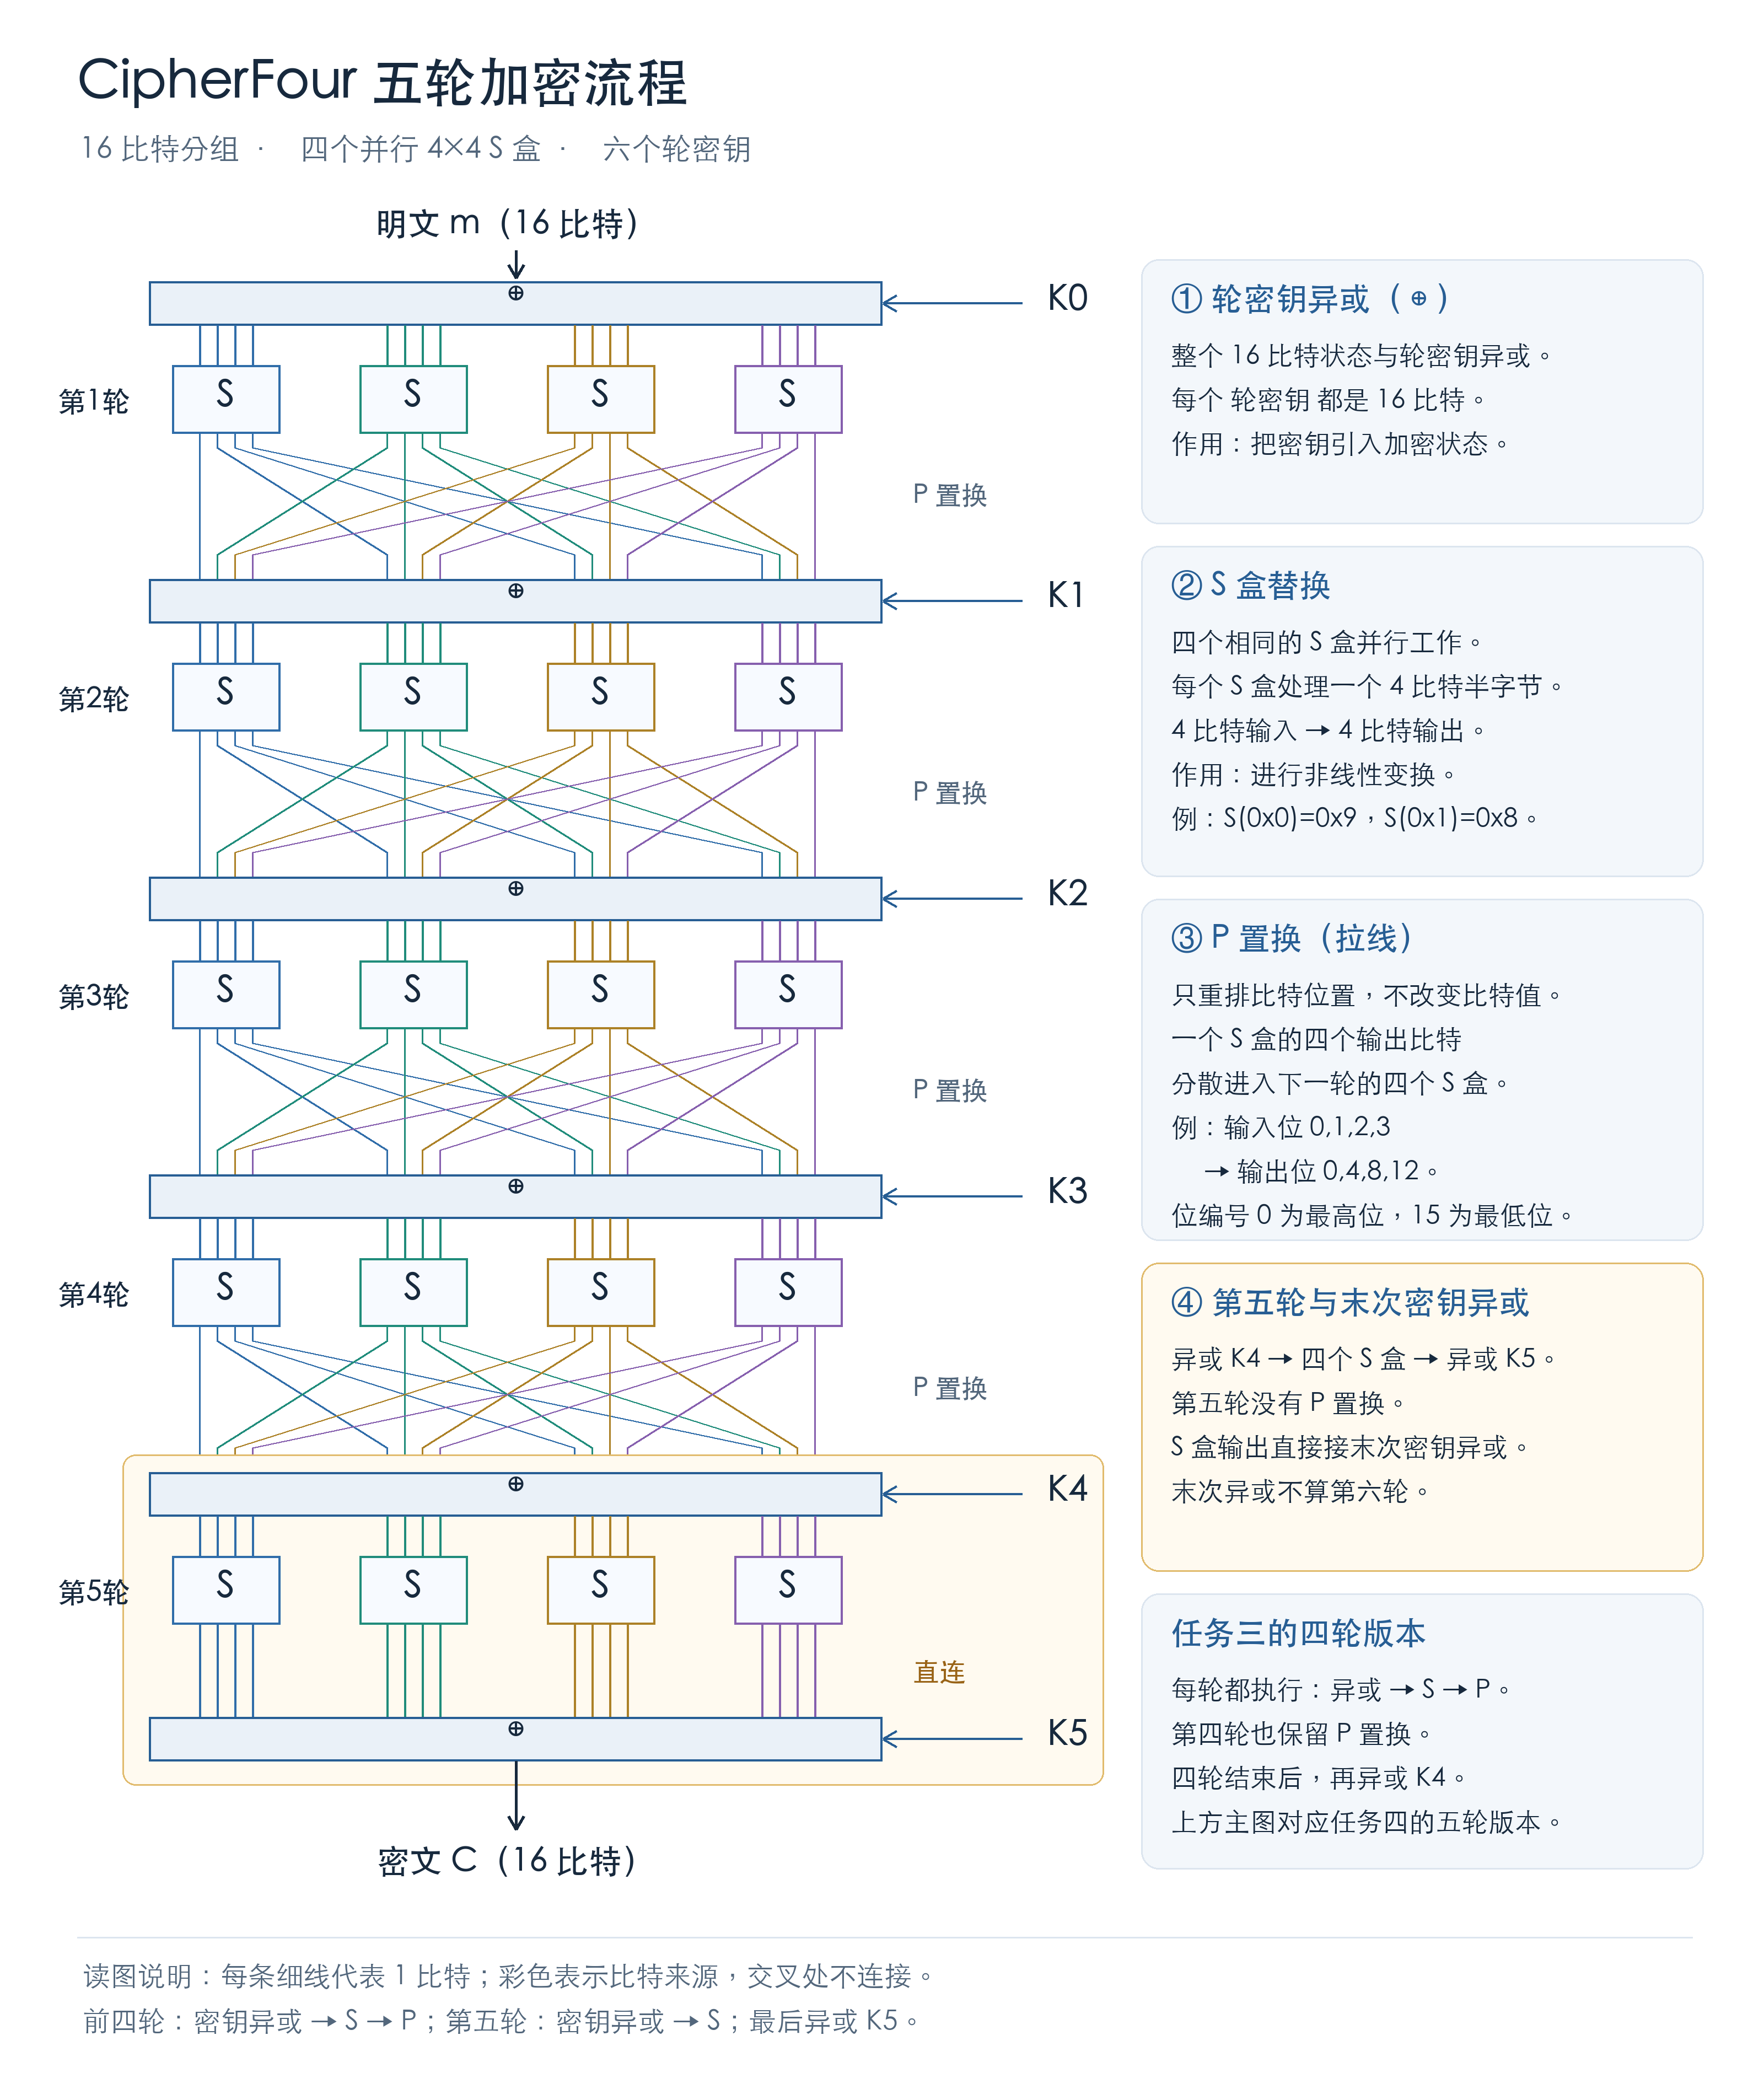
\includegraphics[width=0.85\textwidth]{figures/cipherfour_5round_flow.png}
    \caption{CipherFour算法5轮加密流程图}
    \label{fig:cipherfour_5round_flow}
\end{figure}

\subsection{利用线性规划寻找差分路线}
定义\(B_r(\Delta)\)为经过 \(r\) 轮后，到达差分状态 \(\Delta\) 的所有路线中，概率最大的一条的概率。
对于输入差分，把输入差分为0直接丢掉，因为输入差分为0之后的概率都是1，只能找到全0的路线，定义
\[
B_0(\Delta)=\begin{cases}
1,&\Delta\neq0,\\
0,&\Delta=0.
\end{cases}
\]

沿用书上的符号，假设每一轮的差分为\(\beta_{r}\)

假设已经知道了\(B_{r-1}(\beta_{r-1}),\),现在要计算\(B_r(\beta_{r})\)

从前驱 \(\beta_{r-1}\) 到达 \(\beta_{r}\) 的最佳完整路线概率为
\[
\Pr(\beta_{r-1}\rightarrow \beta_{r})=B_{r-1}(\beta_{r-1})\cdot \Pr(\beta_{r-1},\beta_{r}).
\]

然后再遍历所有前驱，就有

\[
B_r(\beta_{r}) = \max_{\beta_{r-1}}\{B_{r-1}(\beta_{r-1})\cdot \Pr(\beta_{r-1},\beta_{r})\}
\]

这在代码上看是比较简单的，只要遍历所有\(\beta_{r-1}\)就行，\(B_{r-1}(\beta_{r-1}),Pr(\beta_{r-1},\beta_{r})\)知道\(\beta_{r-1}\)后可以直接查表

但是理论上的东西，并不总是可行的，要知道每个\(\beta_{r-1}\)可是有$2^{16}$个，看上去也不是很多，但是注意这里的时间复杂度是在指数上的，也就是\(O(2^{16r})\)

那么如果是4轮，就会达到$2^{64}$,那这就不是一个小数目了，所以要拆分成4个S盒


\subsection{密钥恢复}
\subsubsection{信噪比}
差分分析的密钥恢复阶段中，正确对个数与计数器的平均计数之比称为差分分析的信噪比，记为$S_N$。
设密钥恢复中的高概率差分概率为$p$，可恢复的密钥长度为$k$比特，采样阶段选取$m$对明文，去噪后有$\epsilon m$对保存下来，恢复密钥阶段每个方程平均求得$\eta$个解，则:
$$
S_N = \frac{m \dot p}{\frac{\epsilon m \cdot \eta}{2^k}} = \frac{p \cdot 2^k}{\epsilon \cdot \eta}
$$
\subsubsection{成功率}
成功率即攻击恢复出来的密钥是正确密钥的概率，记为$P_S$。设差分分析中错误密钥的计数器相互独立且均匀分布，若差分概率为$p$，可恢复的密钥长度为$k$比特，采样阶段选$m$对明文，信噪比为$S_N$，计数器前$2^{k-a}$个为正确密钥的候选值，则对足够大的$k$和$m$有：
$$
P_S = \Phi(\frac{\sqrt{pmS_N} - \Phi^{-1}(1-2^{-a})}{\sqrt{S_N+1}})
$$
其中$\Phi$为标准正态分布函数。在以上假设下，要保证成功率为$P_S$，需要的明文对为:
$$
m = \frac{(\sqrt{S_N + 1}\Phi^{-1}(P_S) + \Phi^{-1}(1-2^{-a}))^2 }{S_N}p^{-1}
$$


% 实验内容
\section{任务一}

本任务要求寻找除题目给定差分之外的高概率四轮差分。题目给出的差分为
\[
    (0x0,0x0,0x0,0x1)
    \xrightarrow{\text{4轮}}
    (0x0,0x0,0x0,0x1),
\]
也可以写成
\[
    0x0001\xrightarrow{\text{4轮}}0x0001.
\]

\subsection{直接穷举思路}

对于固定的输入差分 $\alpha$，可以遍历所有 $2^{16}$ 个 16 比特明文 $x$，构造有序明文对 $(x,x\oplus\alpha)$，然后分别进行四轮 CipherFour 加密。若最终密文差分为 $\beta$，则将对应计数加一。因此，固定输入、输出差分的概率为
\[
    P(\alpha\rightarrow\beta)
    =
    \frac{\#\{x:E(x)\oplus E(x\oplus\alpha)=\beta\}}{2^{16}}.
\]

对于每一个非零输入差分，共有 $2^{16}$ 个有序明文对；如果不区分明文对的顺序，则有 $2^{15}$ 个无序明文对。若对全部 $2^{16}-1$ 个非零输入差分都进行穷举，需要处理约 $2^{32}$ 组明文对，计算开销较大。因此，程序使用 S 盒差分分布表（DDT）对差分进行动态规划。

\subsection{S盒差分分布表}

CipherFour 使用一个 4 进 4 出的 S 盒。对于输入差分 $\alpha$ 和输出差分 $\beta$，DDT 定义为
\[
    \mathrm{DDT}[\alpha][\beta]
    =
    \#\left\{x\in\{0,1,\ldots,15\}:
    S(x)\oplus S(x\oplus\alpha)=\beta\right\}.
\]

因此，单个 S 盒的差分传播概率为
\[
    T[\alpha][\beta]
    =
    \frac{\mathrm{DDT}[\alpha][\beta]}{16}
    =
    \frac{\mathrm{DDT}[\alpha][\beta]}{2^4}.
\]

代码中的 DDT 计算如下：
\begin{lstlisting}
for diff_in in range(16):
    for value in range(16):
        diff_out = S[value] ^ S[value ^ diff_in]
        diff_table[diff_in][diff_out] += 1
\end{lstlisting}

其中，\texttt{diff\_table[diff\_in][diff\_out]} 保存输入差分为 \texttt{diff\_in}、输出差分为 \texttt{diff\_out} 的出现次数。

\subsection{一轮差分传播}

一个 16 比特差分可以拆成四个半字节：
\[
    \Delta=(a_0,a_1,a_2,a_3).
\]

若四个 S 盒的输出差分为
\[
    \Gamma=(b_0,b_1,b_2,b_3),
\]
则在固定当前差分的条件下，四个 S 盒同时发生该传播的概率为
\[
    Q(\Delta,\Gamma)
    =
    \prod_{i=0}^{3}T[a_i][b_i].
\]

例如，输入差分 $0x0001=(0,0,0,1)$ 时，前三个 S 盒的输入差分为 0，并且
\[
    T[0][0]=1.
\]
只有最后一个 S 盒产生分支。对于本实验使用的 S 盒，输入差分 1 可以传播为输出差分 1、2、5，其概率分别为 $1/2$、$1/4$、$1/4$。因此，经过 S 盒层后可能得到
\[
    0x0001\ (1/2),\qquad
    0x0002\ (1/4),\qquad
    0x0005\ (1/4).
\]

代码中的 \texttt{score} 保存四个半字节的联合概率分布，其形状为
\[
    (\text{batch},16,16,16,16).
\]
处理某一个半字节时，程序计算
\[
    F_{\mathrm{new}}(\beta)
    =
    \sum_{\alpha=0}^{15}
    F_{\mathrm{old}}(\alpha)T[\alpha][\beta].
\]

这对应代码中的矩阵乘法：
\begin{lstlisting}
score_matrix = moved_score.reshape(-1, 16)
updated_score = score_matrix @ probability_table
\end{lstlisting}

程序依次处理四个 S 盒：
\begin{lstlisting}
for position in range(4):
    score = update_one_sbox_distribution(
        score, probability_table, position
    )
\end{lstlisting}

对于一个确定的当前 16 比特差分，这一过程等价于四个 S 盒概率的乘积；当当前状态本身是多个差分状态的概率混合时，程序还会对所有前驱状态的概率进行求和，因此需要保存四个半字节的联合分布，而不能只分别保存四个边缘概率。

四个 S 盒处理完成后，将得到的 16 比特差分经过 P 置换。代码预先计算所有 16 比特状态的置换结果：
\begin{lstlisting}
permutation = np.array(
    [P_box(value) for value in range(STATE_SIZE)],
    dtype=np.int32,
)
\end{lstlisting}

由于 P 是比特置换，满足
\[
    P(X)\oplus P(Y)=P(X\oplus Y),
\]
因此可以直接对差分状态进行 P 置换。经过 P 置换后的差分分布作为下一轮的输入。

\subsection{四轮动态规划}

设初始输入差分为 $\alpha$，经过 $r$ 轮后的差分分布为 $D_r^{(\alpha)}$。初始时只有输入差分本身的概率为 1：
\[
    D_0^{(\alpha)}(\Delta)=
    \begin{cases}
        1,&\Delta=\alpha,\\
        0,&\Delta\ne\alpha.
    \end{cases}
\]

代码通过以下语句完成初始化：
\begin{lstlisting}
score[rows, nibble0, nibble1, nibble2, nibble3] = 1.0
\end{lstlisting}

记一轮四个 S 盒和 P 置换的差分转移概率为 $R(\Delta,\Delta')$，则每轮动态规划满足
\[
    D_{r+1}^{(\alpha)}(\Delta')
    =
    \sum_{\Delta}
    D_r^{(\alpha)}(\Delta)R(\Delta,\Delta').
\]

因此，四轮后的输出差分概率为
\[
    D_4^{(\alpha)}(\beta)
    =
    \sum_{\Delta_1,\Delta_2,\Delta_3}
    R(\alpha,\Delta_1)
    R(\Delta_1,\Delta_2)
    R(\Delta_2,\Delta_3)
    R(\Delta_3,\beta).
\]

这个求和包含了从输入差分 $\alpha$ 到输出差分 $\beta$ 的所有差分路线。代码的外层循环对应四轮传播：
\begin{lstlisting}
for _ in range(NUMBER_OF_ROUNDS):
    for position in range(4):
        score = update_one_sbox_distribution(
            score, probability_table, position
        )

    after_sbox = score.reshape(batch_size, STATE_SIZE)
    after_pbox[:, permutation] = after_sbox
    score = after_pbox.reshape(
        batch_size, 16, 16, 16, 16
    )
\end{lstlisting}

这里每一轮的输入和输出都是 16 比特差分状态的概率分布，不是具体的明文或密文。四轮循环结束后，\texttt{score} 中保存每个输入差分经过四轮后得到所有输出差分的概率。

\subsection{高概率差分的搜索}

程序从 \texttt{0x0001} 到 \texttt{0xFFFF} 遍历全部 $2^{16}-1$ 个非零输入差分，并将输入差分按 32 个一批进行处理，以降低内存开销。分批处理不会减少搜索范围。

对于每个输入差分 $\alpha$，四轮动态规划得到所有输出差分 $\beta$ 的概率分布。程序使用
\begin{lstlisting}
output_differences = np.argmax(
    output_distribution, axis=1
)
\end{lstlisting}
找到该输入差分对应的最大概率输出差分。随后，再在所有输入差分对应的候选结果中选择全局最大值。

题目要求排除 $0x0001\rightarrow0x0001$，因此代码只对输入差分 \texttt{0x0001} 的输出分布执行：
\begin{lstlisting}
candidate_distribution[
    EXCLUDED_OUTPUT_DIFFERENCE
] = 0.0
\end{lstlisting}
然后重新选择该输入差分对应的最佳输出差分。

\begin{figure}[H]
    \centering
    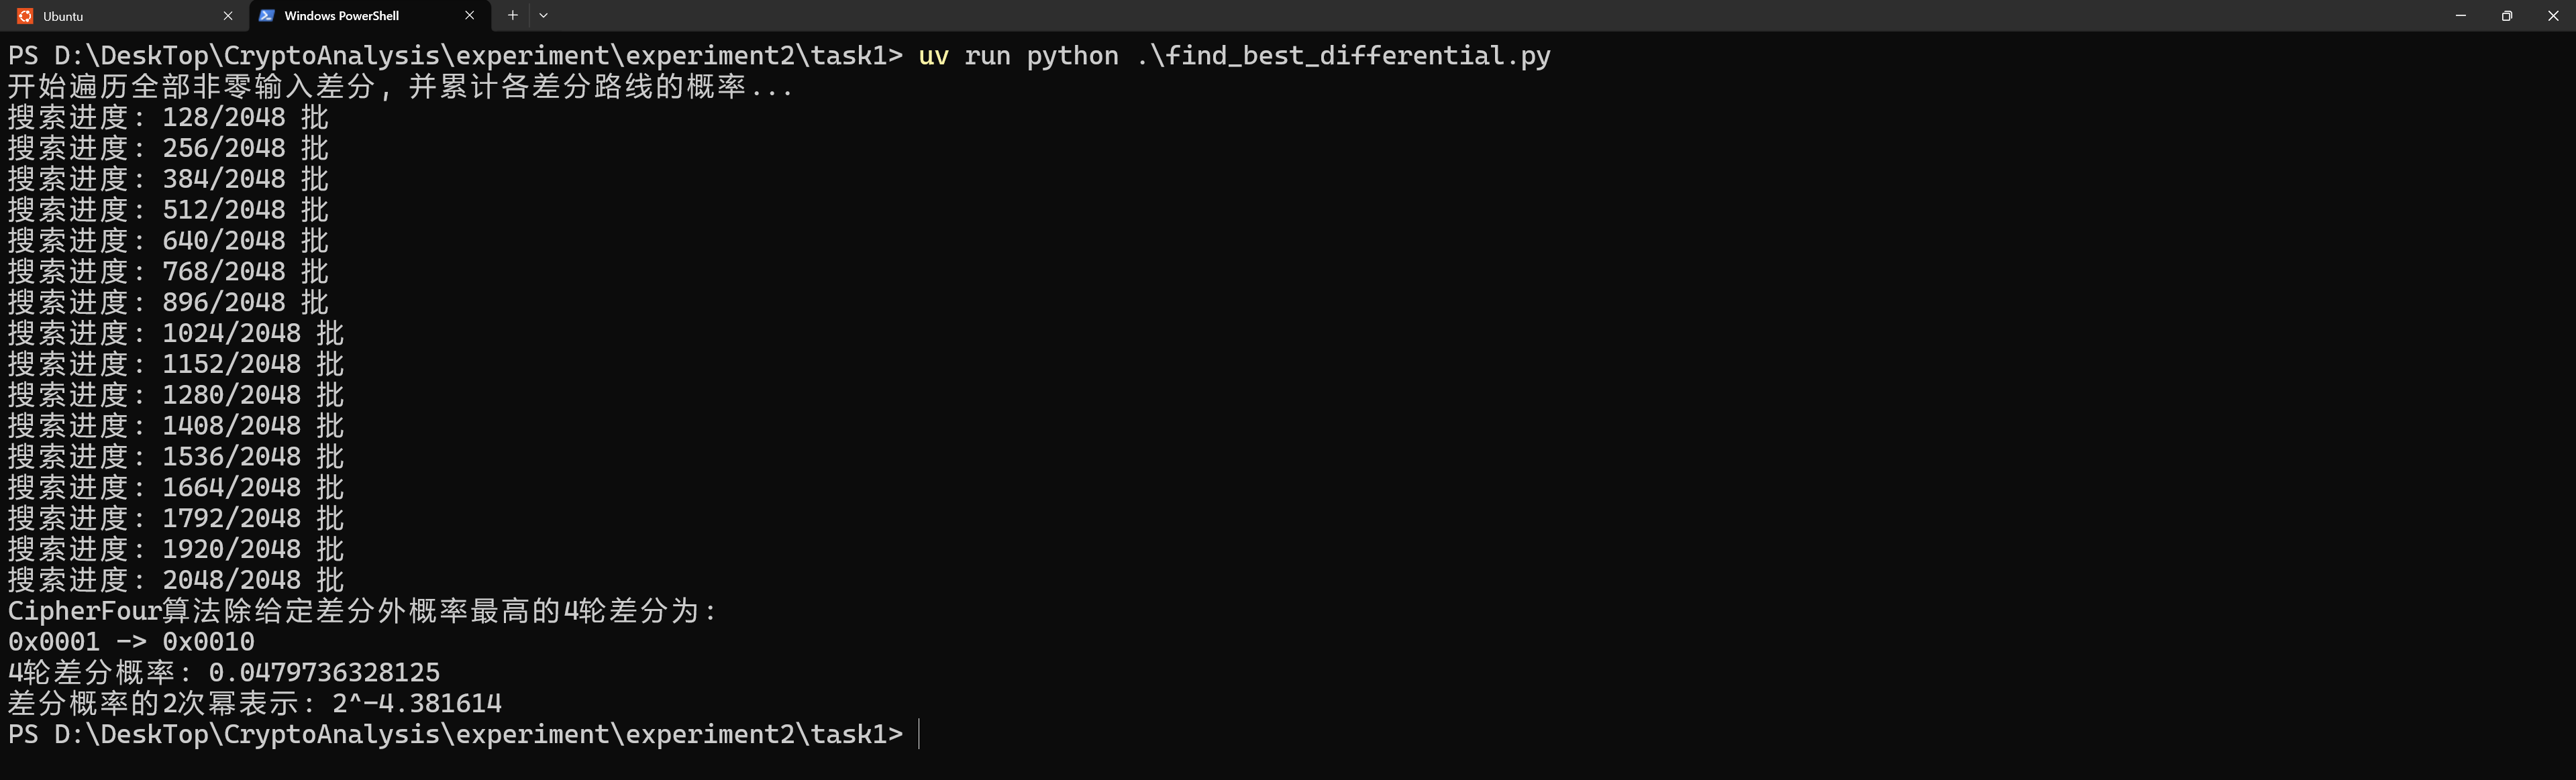
\includegraphics[width = 1\textwidth]{figures/task1_diffeientrial.png}
    \caption{寻找高概率差分}
\end{figure}

程序最终找到的四轮高概率差分为
\[
    (0x0,0x0,0x0,0x1)
    \longrightarrow
    (0x0,0x0,0x1,0x0),
\]
即
\[
    0x0001\longrightarrow0x0010.
\]

其基于 DDT 动态规划得到的四轮差分概率为
\[
    P(0x0001\rightarrow0x0010)
    =0.0479736328125
    \approx 2^{-4.381614}.
\]

这里计算的是连接相同输入、输出差分的所有差分路线的概率总和，而不是某一条单独差分路线的概率。后续任务二再通过枚举具体明文对，统计该输入、输出差分在固定 CipherFour 置换网络中的实际路线和频率。
\subsection{方法二：排除最优路线后的搜索}

示例程序搜索的是概率最高的单条四轮差分路线。设 $\Delta_0$ 为输入差分，$\Delta_r$ 为第 $r$ 轮经过 S 盒和 P 置换后的差分，则一条路线写为
\[
    \Delta_0\rightarrow\Delta_1\rightarrow\Delta_2
    \rightarrow\Delta_3\rightarrow\Delta_4.
\]
程序得到的最优路线为
\[
    \text{0x}0001\rightarrow\text{0x}0001
    \rightarrow\text{0x}0001\rightarrow\text{0x}0001
    \rightarrow\text{0x}0001,
\]
每轮传播概率均为 $1/2$，所以该路线的概率为 $(1/2)^4=1/16$。为了判断是否存在概率相同的其他路线，需要在搜索中排除这条已知路线。

\subsubsection{排除路线的依据}

设 $B_r(\Delta)$ 表示经过 $r$ 轮后到达差分状态 $\Delta$ 的最大单条路线概率。一轮差分转移概率仍记为 $R(u,v)$，则示例程序的更新规则可写为
\[
    B_{r+1}(v)=\max_u\bigl\{B_r(u)R(u,v)\bigr\}.
\]
这里取最大值，与方法一中对所有前驱路线求和不同。初始化时，所有非零输入差分的 $B_0$ 均设为 $1$，而 $B_0(0)=0$。这是因为零输入差分会以概率 $1$ 沿全零路线传播；将其排除，才能搜索非零差分路线。

原最优路线在 $\Delta_0,\ldots,\Delta_4$ 的五个位置上均为 $\text{0x}0001$。任意另一条路线至少有一个位置与之不同，因此可以分别在位置 $j=0,1,2,3,4$ 禁用差分 $\text{0x}0001$，对五次搜索结果取最大概率。五个受限搜索覆盖了所有不同于原最优路线的路线；某条路线若在多个位置不同，也可能在多次搜索中重复出现。

实现时，$j=0$ 对应将初始概率数组的 $\text{0x}0001$ 项置零；$j=1,\ldots,4$ 对应在第 $j$ 轮完成 S 盒和 P 置换后，将 $B_j(\text{0x}0001)$ 置零。每次四轮搜索结束后，再由最终状态逆向追溯各轮差分，得到完整路线。图~\ref{fig:task1_method2_code} 展示了代码中的位置参数和禁用操作。

\begin{figure}[H]
    \centering
    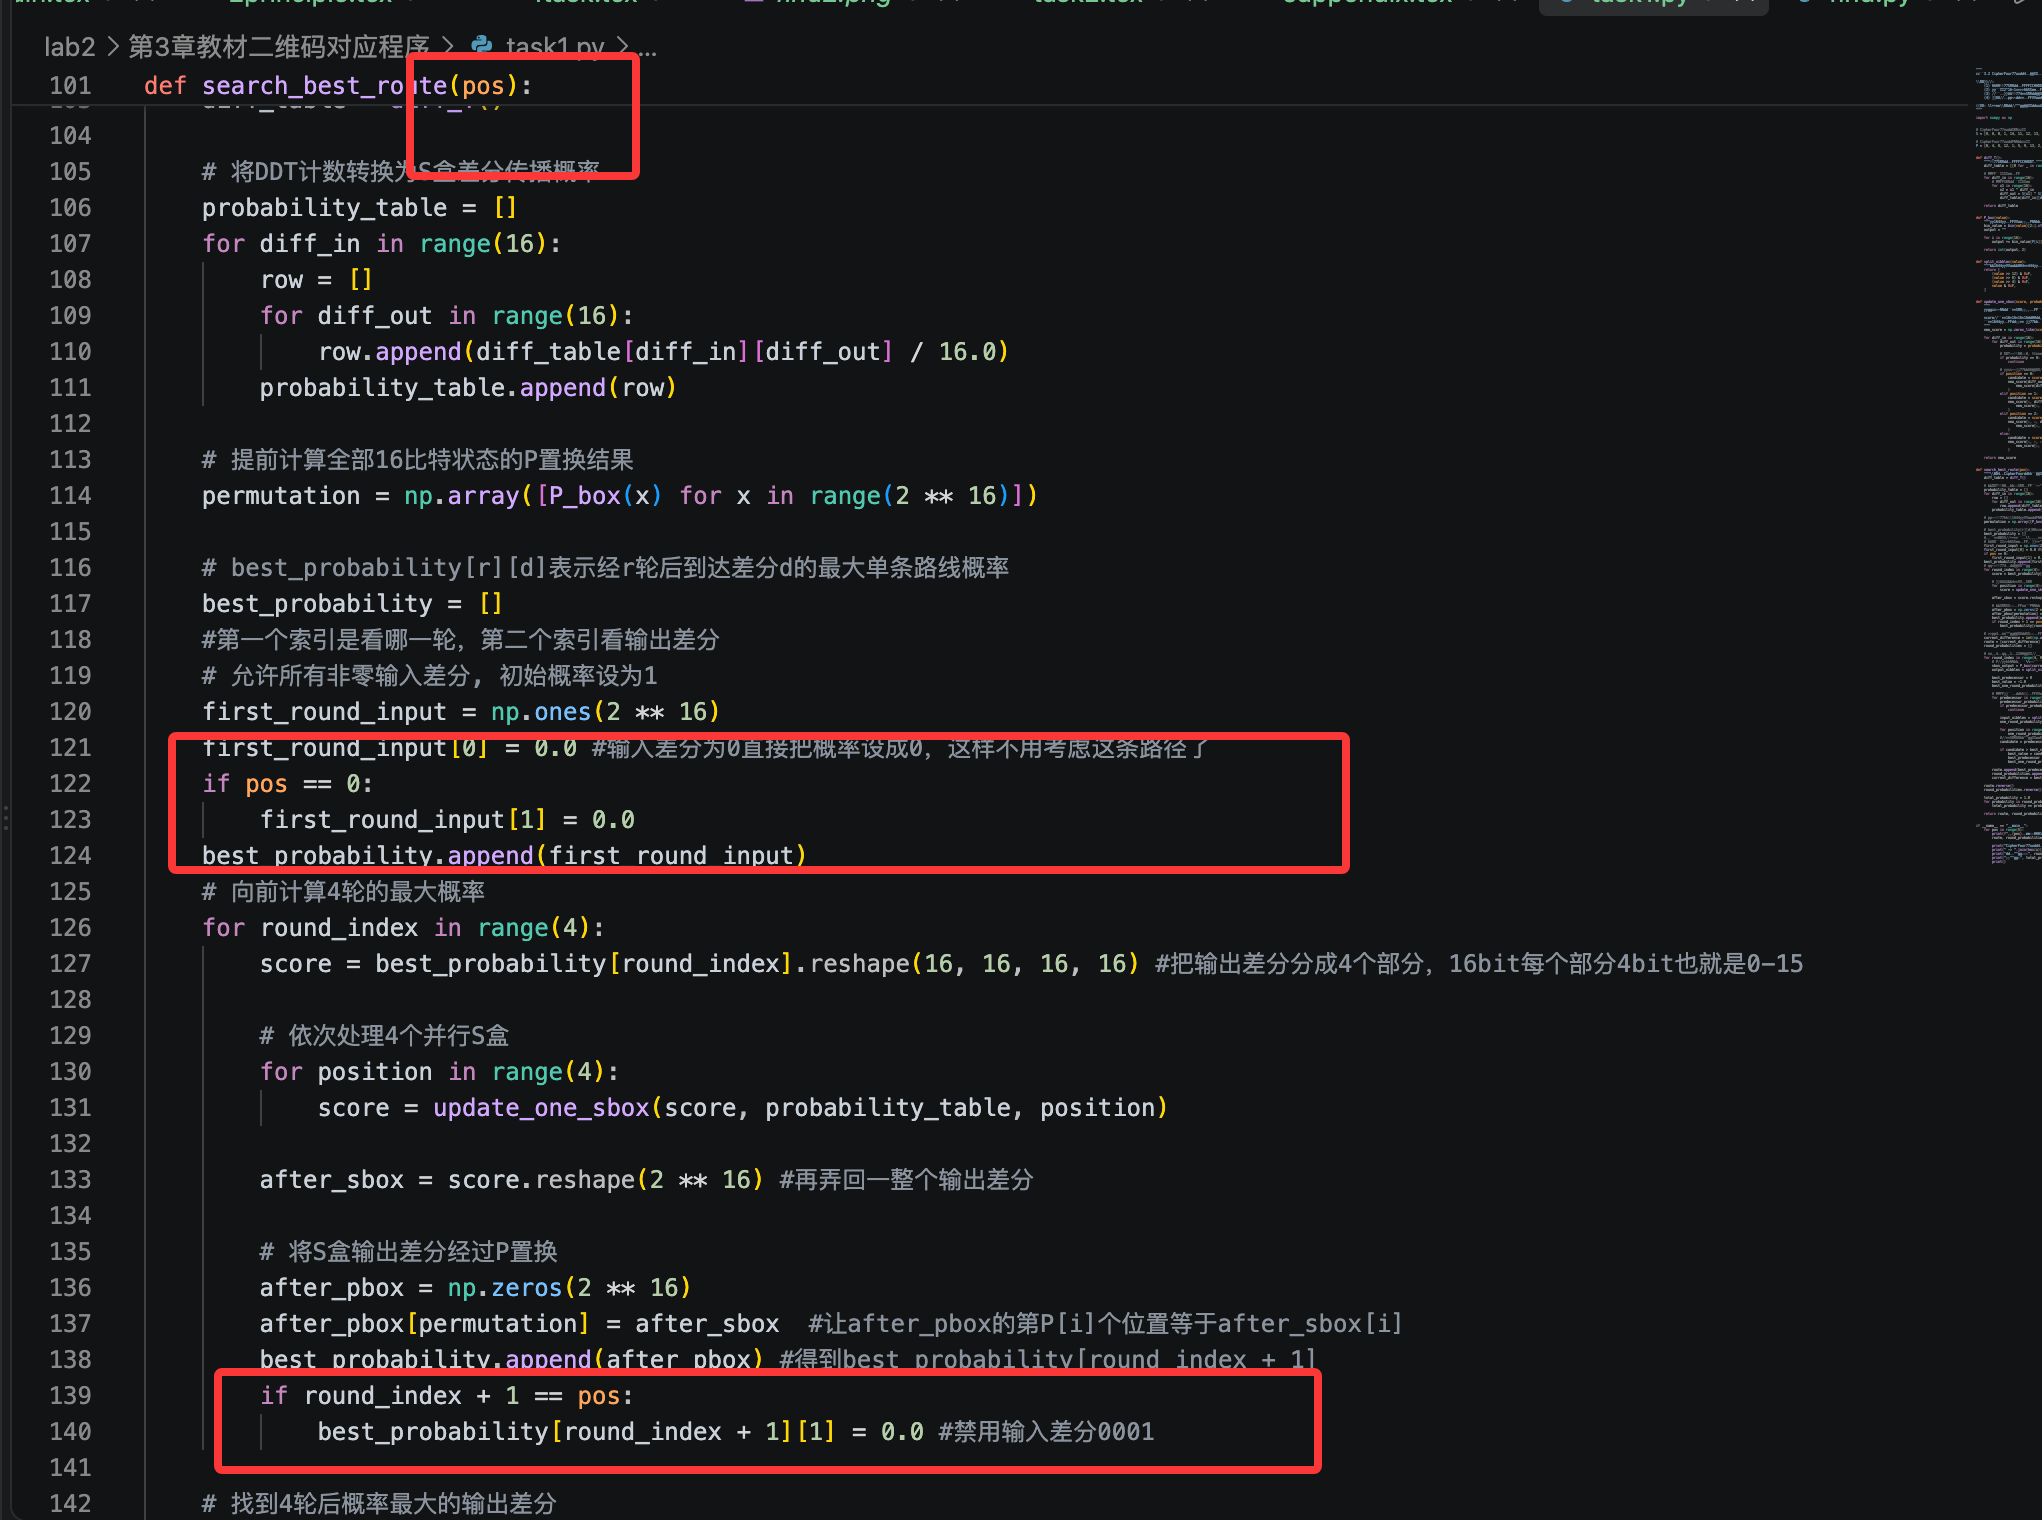
\includegraphics[width=0.8\textwidth]{figures/task1_enhance.png}
    \caption{在指定位置排除已知最优路线的差分状态}
    \label{fig:task1_method2_code}
\end{figure}

\subsubsection{搜索结果}

图~\ref{fig:task1_method2_result} 给出五次受限搜索的输出。表~\ref{tab:task1_method2_result} 将各路线整理为十六进制差分状态序列，并按四轮概率的乘积给出路线概率。

\begin{figure}[H]
    \centering
    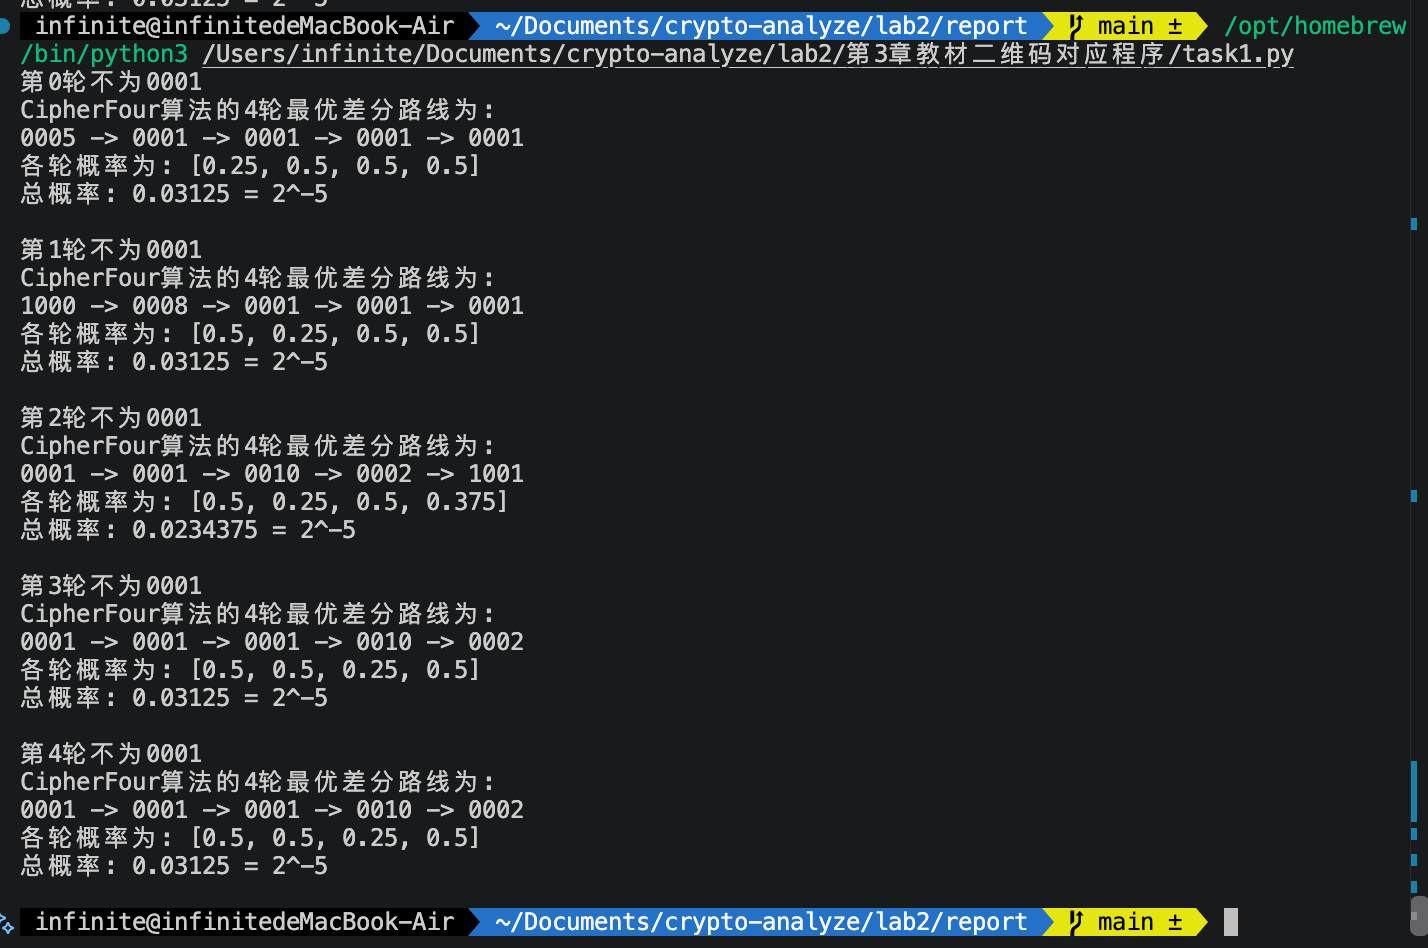
\includegraphics[width=0.8\textwidth]{figures/task1_result.png}
    \caption{分别禁用五个位置后的差分路线搜索结果}
    \label{fig:task1_method2_result}
\end{figure}

\begin{table}[H]
    \centering
    \small
    \caption{排除已知最优路线后得到的差分路线}
    \label{tab:task1_method2_result}
    \renewcommand{\arraystretch}{1.15}
    \begin{tabular}{ccl}
        \toprule
        禁用位置 $j$ & 路线概率 & 差分路线（十六进制） \\
        \midrule
        0 & $1/32$ & $0005\to0001\to0001\to0001\to0001$ \\
        1 & $1/32$ & $1000\to0008\to0001\to0001\to0001$ \\
        2 & $3/128$ & $0001\to0001\to0010\to0002\to1001$ \\
        3 & $1/32$ & $0001\to0001\to0001\to0010\to0002$ \\
        4 & $1/32$ & $0001\to0001\to0001\to0010\to0002$ \\
        \bottomrule
    \end{tabular}
\end{table}

在禁用位置 $j=2$ 的一次搜索中，四轮概率分别为 $1/2,1/4,1/2,3/8$，实际乘积为 $3/128=0.0234375$。截图末尾的 $2^{-5}$ 是程序对概率取对数后再转为整数的显示结果，不能作为这条路线的精确概率。其余四次受限搜索均得到 $1/32$。因此，排除原最优路线后，概率最高的单条路线为 $1/32$，低于原路线的 $1/16$；位置 $j=3$ 与 $j=4$ 搜索到了同一条路线，五次结果共对应四条不同路线。

这些结果反映的是单条差分路线的概率。若只看输入、输出差分，上述四条路线分别对应 $\text{0x}0005\to\text{0x}0001$、$\text{0x}1000\to\text{0x}0001$、$\text{0x}0001\to\text{0x}1001$ 和 $\text{0x}0001\to\text{0x}0002$。同一输入、输出差分还可能由其他路线实现，因此这些路线概率不能直接当作对应差分的总概率；差分总概率应按方法一对所有路线求和。


\section{任务二}
根据任务一找到的新4轮高概率差分，要寻找所有对应的差分路线，思路为遍历所有$2^{16}$种输入差分对，即$x \in \{0,1,\dots2^{16} - 1\}$、$x' = x\oplus \Delta_{in}$，
记录下4轮加密过程中每一轮的中间异或结果，当满足输出差分$y \oplus y' = \Delta_{out}$时，该路线即为所要求的4轮差分的差分路线，将该路线记录下来，最后输出所有差分路线并计算概率(注意这里按照输入是有序对时共$2^{16}$种满足条件的差分对，若按照无序对考察，则差分路线和总的差分对数量均减半，但最终概率不变)，计算概率为:
$$
P = \frac{\# \{x:F^4(x) \oplus F^4(x \oplus \Delta_{in}) = \Delta_{out}\} }{2^{16}}
$$
按照上述思路编写代码，运行结果如下:
\begin{figure}[H]
    \centering
    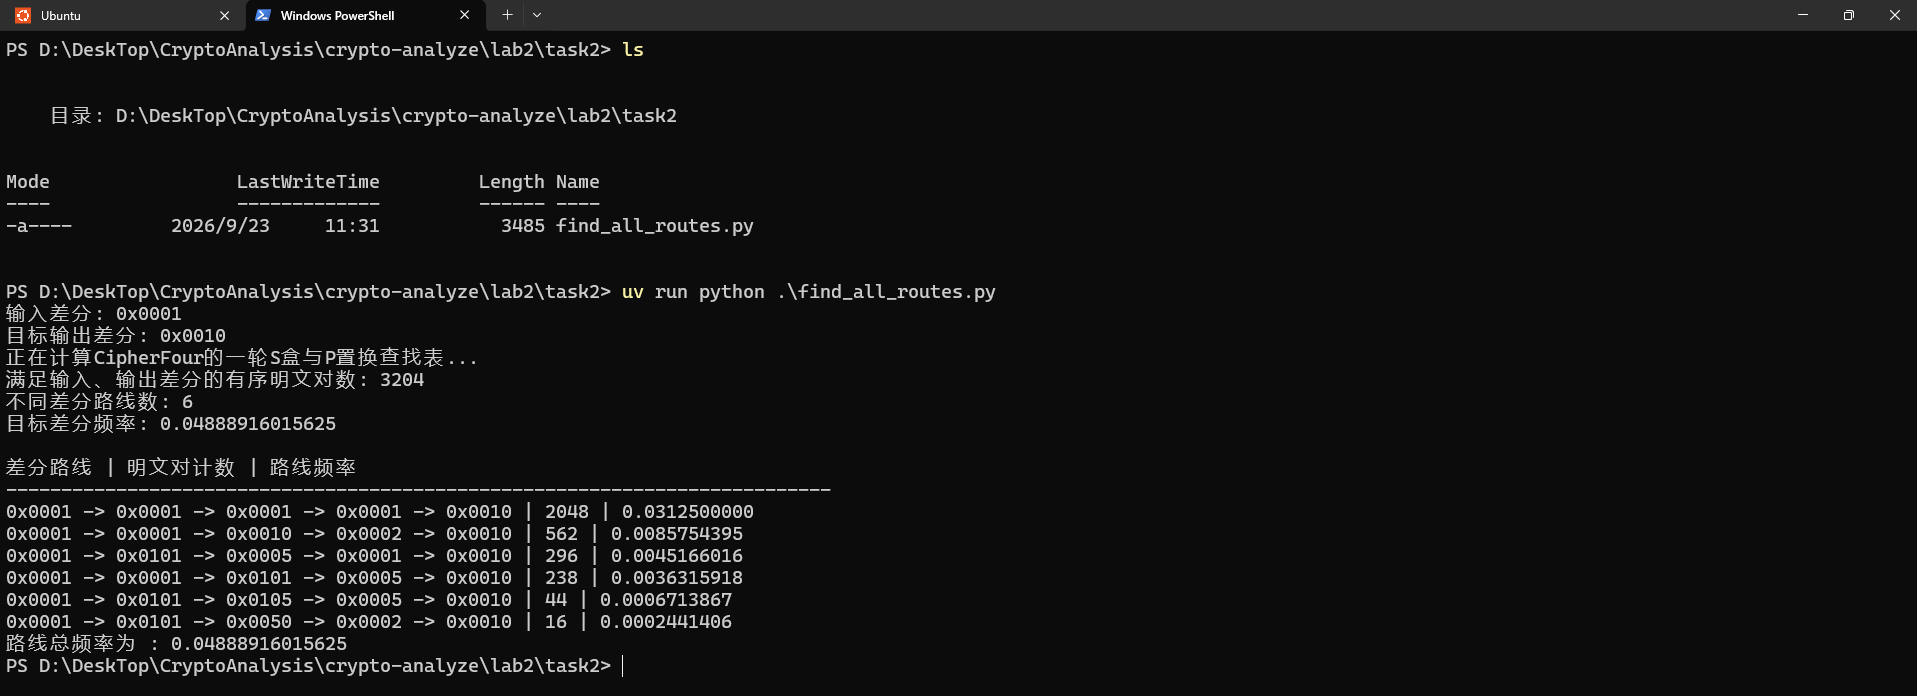
\includegraphics[width = 1\textwidth]{figures/task2_routes.png}
    \caption{所有新4轮差分路线}
\end{figure}

\input{content/task3/task3_1.tex}
\input{content/task4/task4_1.tex}
\input{content/task5/task5.tex}

\section{实验总结}

\clearpage
\appendix
\section{实验代码}
见代码附录文件。% 不在实验报告中展示具体代码，反正都会教代码压缩包
% 本附录列出本次实验中使用的 Enigma 加密及性能测试程序。

% \subsection{寻找差分路线}
% \lstinputlisting[caption={.py}]{../code/task1.py}

% \subsection{Enigma 密钥恢复程序}
% \lstinputlisting[caption={decrypt.py}]{../decrypt.py}
\section{实验报告完整地址}
实验完整代码、实验报告 \LaTeX{} 源代码见仓库：
\url{https://github.com/infinitepwn/crypto-analyze.git}


\section{AI使用情况}
本实验使用AI辅助编程和实验报告的排版、错别字检查，实验主体流程设计、结果分析和实验报告的撰写未使用AI。

\end{document}
